\documentclass{article}

\usepackage{amsmath}
\usepackage{pgfplots}  
\usepackage{titling} 
\usepackage[utf8x]{inputenc}
\usepackage{lmodern,textcomp} 

\pgfplotsset{compat=newest}

\title{Actividad en Clase \\ Programacion Lineal}
\author{Nathan Alspaugh \\ Colegio Real Royal School}

\begin{document}
\maketitle
\newtheorem{linalprogramming}{Problema}
\begin{linalprogramming}
    Una fabrica tiene 2 tipos de joyas. La unidad del tipo A se hace con 1g de oro y 1.5y de plata y se vende a 25€. L de tipo B se vende a 30€ y lleva 1.5g de oro y 1g de plata. Si solo dispone 750 de cada metal, cuantas joyas hace la fabrica de cada tipo para maximizar los ingresos?
    \begin{equation}
        \begin{aligned}
            & \text{x seria cantidad del tipo A} \\
            & \text{y seria cantidad del tipo B }
        \end{aligned}
    \end{equation}
    \begin{equation}
        \begin{tabular}{|c | c | c | c|} 
            \hline
             & A & B & Max \\
            \hline
            Oro & 1g & 1.5g & 750g \\ 
            \hline
            Plata & 1.5g & 1g & 750g \\
            \hline
            Precio & €20 & €30 &  \\
            \hline
           \end{tabular}
\end{equation}
    \begin{equation}
        \begin{aligned}
           & x \geq 0; \land y \geq 0; \\
            & x + 1.5y \leq 750 \\
            & 1.5x + y \leq 750
        \end{aligned}
    \end{equation}
    \begin{equation}
            F(x, y) = 20x + 30y
    \end{equation}
    \begin{equation}
        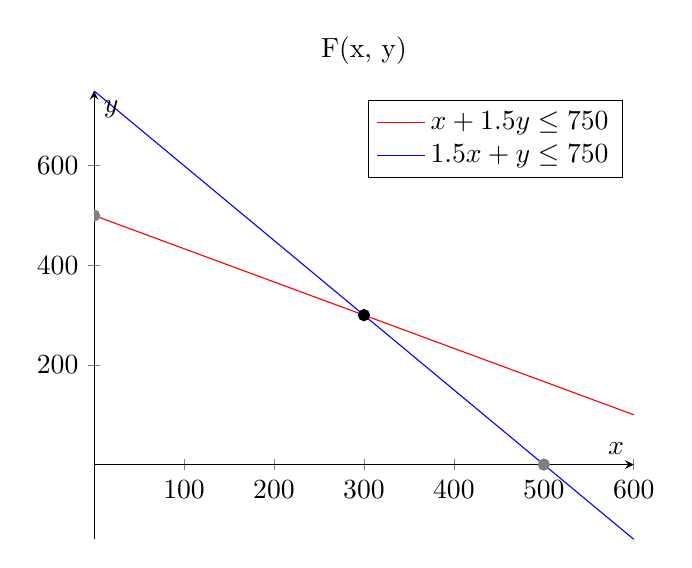
\begin{tikzpicture} 
            \begin{axis}[axis lines=middle,xlabel=$x$,ylabel=$y$,title={F(x, y)}]
                
                \addplot [
domain=0:600, 
samples=100, 
color=red,
]
{(750-x)/1.5};
\addlegendentry{\(x + 1.5y \leq 750\)}
%Here the blue parabola is defined
\addplot [
domain=0:600, 
samples=100, 
color=blue,
]
{(750-1.5*x)};
\addlegendentry{\(1.5x + y \leq 750\)}
\filldraw[black] (300,300) circle (2pt);
\filldraw[gray] (0, 500) circle (2pt);
\filldraw[gray] (500, 0) circle (2pt);
            \end{axis}
        \end{tikzpicture} 
\end{equation}
    \begin{equation}
        \begin{tabular}{|c | c | c|} 
            \hline
            x & y & F(x, y) \\
            \hline
            500 & 0 & 12500 \\ 
            \hline
            0 & 500 & 15000 \\
            \hline
            300 & 300 & 16500 \\
            \hline
           \end{tabular}
    \end{equation}
    \begin{equation}
        \begin{aligned}
            \text{Para } x = 500 \land y = 0 \\
            F(x, y) & = 25x + 30y \\
            F(500, 0) & = 25(500) + 30(0) \\
            F(500, 0) & = 12500
        \end{aligned}
    \end{equation}
    \begin{equation}
        \begin{aligned}
            \text{Para } x = 0 \land y = 500 \\
            F(x, y) & = 25x + 30y \\
            F(0, 500) & = 25(0) + 30(500) \\
            F(0, 500) & = 15000
        \end{aligned}
    \end{equation}
    \begin{equation}
        \begin{aligned}
            \text{Para } x = 300 \land y = 300 \\
            F(x, y) & = 25x + 30y \\
            F(300, 300) & = 25(300) + 30(300) \\
            F(300, 300) & = 16500
        \end{aligned}
    \end{equation}
    \begin{equation}
        \text{El maximo del funccion es en el punto } (300, 300) 
    \end{equation}
\end{linalprogramming}

\end{document}